%%%%%%%%%%%%%%%%%%%%%%%%%%%%%%%%%%%%%%%%%%%%%%%%%%%%%
%
%
%  	DYNAMICAL MODELS - ODEs, Systems of ODEs, Bifurcation, PDEs, 
%
%
%%%%%%%%%%%%%%%%%%%%%%%%%%%%%%%%%%%%%%%%%%%%%%%%%%%%%

\begin{slide}
\question

\begin{slidesonly}
	\vspace{3cm}
\end{slidesonly}

\begin{center}
\Huge 
\textcolor{LimeGreen}{Dynamical Models}
\end{center}

	
\end{slide}








%
%\begin{slide}
%
%\question
%	The tree model
%	\begin{align*}
%		H'(t) &= 0.3\cdot A(t)-b\cdot H(t)\\
%		A'(t) &= -0.3\cdot (H(t))^2 + A(t)
%	\end{align*}
%	was based on the premises
%	\begin{itemize}[leftmargin=3em]
%		\item[ $P_{\text{height 1}}$] CO$_2$ is absorbed by the leaves and turned directly into trunk height.
%		\item[ $P_{\text{height 2}}$] The tree is in a swamp and constantly sinks at a speed proportional to its height.
%		\item[ $P_{\text{leaves 1}}$] Leaves grow proportionally to the energy available.
%		\item[ $P_{\text{energy 1}}$] The tree gains energy from the sun proportionally to the leaf area.
%		\item[ $P_{\text{energy 2}}$] The tree loses energy proportionally to the square of its height.
%	\end{itemize}
%
%	\begin{parts}
%		\item How are the premises expressed in the differential equations?
%		\item What does the parameter $b$ represent (in the real world)?
%
%		\item 
%	\end{parts}
%	
%\end{slide}
%


\addcontentsline{toc}{subsection}{Modelling with ODEs}


\begin{slide}

\question

\begin{center}
	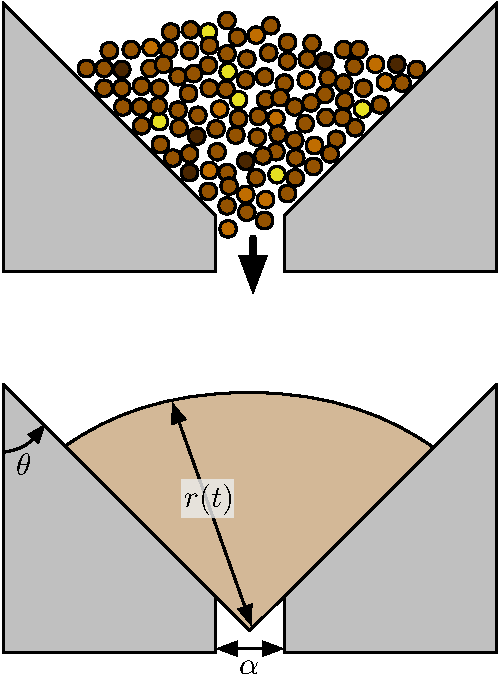
\includegraphics[width=145pt]{images/stadium.pdf}
\end{center}

	The following ordinary differential equation models a crowd leaving a stadium through an exit
	\[
	2 \theta r \frac{dr}{dt_{}} = - k \alpha \sqrt{r}
	\]
	
\begin{slidesonly}
	\bigskip
\end{slidesonly}

	
	based on the premise \\[-20pt]
	\begin{itemize}
		\item[(TL)]	Torricelli's Law: The area of the region occupied by the crowd decreases proportionally to the width of the exit times the square root of its radius. %\\[-20pt]
	\end{itemize}

	\begin{parts}
		\item How is the premise expressed in the differential equation?
		\item Sketch a slope field for this model

			\url{https://www.desmos.com/calculator/lxb4g6cuiz}

		and use it to study how the time it would take to evacuate that section depends on the parameters.
		
		\item Using Euler's method, estimate how long it would take to evacuate a stadium with $\alpha=k=1$, $\theta=\frac{\pi}{5}$ and $r(0)=2$.
		
%		\url{https://www.desmos.com/calculator/2dfs5s1axi}
\end{parts}

\end{slide}


\begin{slide}

\question

\begin{center}
	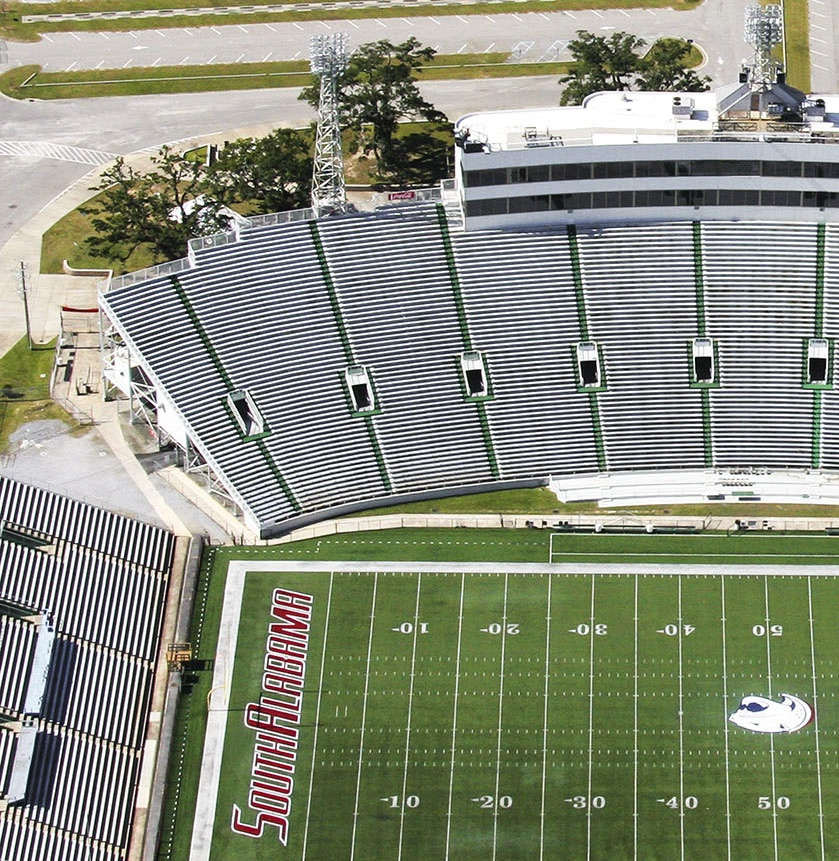
\includegraphics[width=.4\textwidth]{images/Ladd_Stadium-cropped.jpg}
	
	Ladd Peebles Stadium
\end{center}

\begin{slidesonly}
	\bigskip
\end{slidesonly}

According to the paper \href{https://www.researchgate.net/publication/289492130_A_study_of_stadium_exit_design_on_evacuation_performance}{\tt ``A study of stadium exit design on evacuation performance''} studying the Ladd Peebles stadium:
\begin{itemize}
	\item The average person occupies 0.15m$^2$.
	\item The stadium fits 1200 people in one section.
	\item The exits are 1.5m wide.
\end{itemize}


\begin{parts}
	\item According to an experiment in the paper, it took 8 minutes to evacuate the stadium. Use this to estimate $k$ for Ladd Peebles.
	
	\item In the same paper, ``for safety, the maximum flow through an exit is 109 people per meter-width per minute.'' Does Ladd Peebles satisfy this safety concern?

\end{parts}

\end{slide}

\begin{solution}
\begin{slide}

\textbf{Solution:}

\begin{itemize}
\item $\theta r^2(0) = 1200 \cdot (0.15) \quad \Rightarrow \quad r(0) \approx 7.6m$
\item $\theta = \pi$
\item $\alpha = 1.5$
\item To get everyone out in 8 minutes $\Rightarrow k = 7.33$ (time units are minutes)
\item $p(t) = A\big(r(t)\big)/(0.15\cdot 1.5) = $ people per meter-width
\item $p(t) = 2\theta \frac12 r^2(t)/(0.15\cdot 1.5) = \frac{\theta}{0.225} r^2(t)$
\item $\displaystyle p'(t) = \frac{1}{0.225} \underbrace{2 \theta r\frac{dr}{dt}}_{- k \alpha \sqrt{r}} = -\frac{k \alpha}{0.225} \sqrt{r(t)} = - \frac{152}{3} \sqrt{r(t)}$ 
\item Max at $t=0$ when $|p'(t)| \approx 139.678$
\item The solution is here: \href{https://utoronto.syzygy.ca/jupyter/user-redirect/git-pull?repo=https://github.com/bigfatbernie/IBLMathModeling&subPath=book/python/Stadium-Euler.ipynb}{\tt Stadium-Euler.ipynb}
\end{itemize}

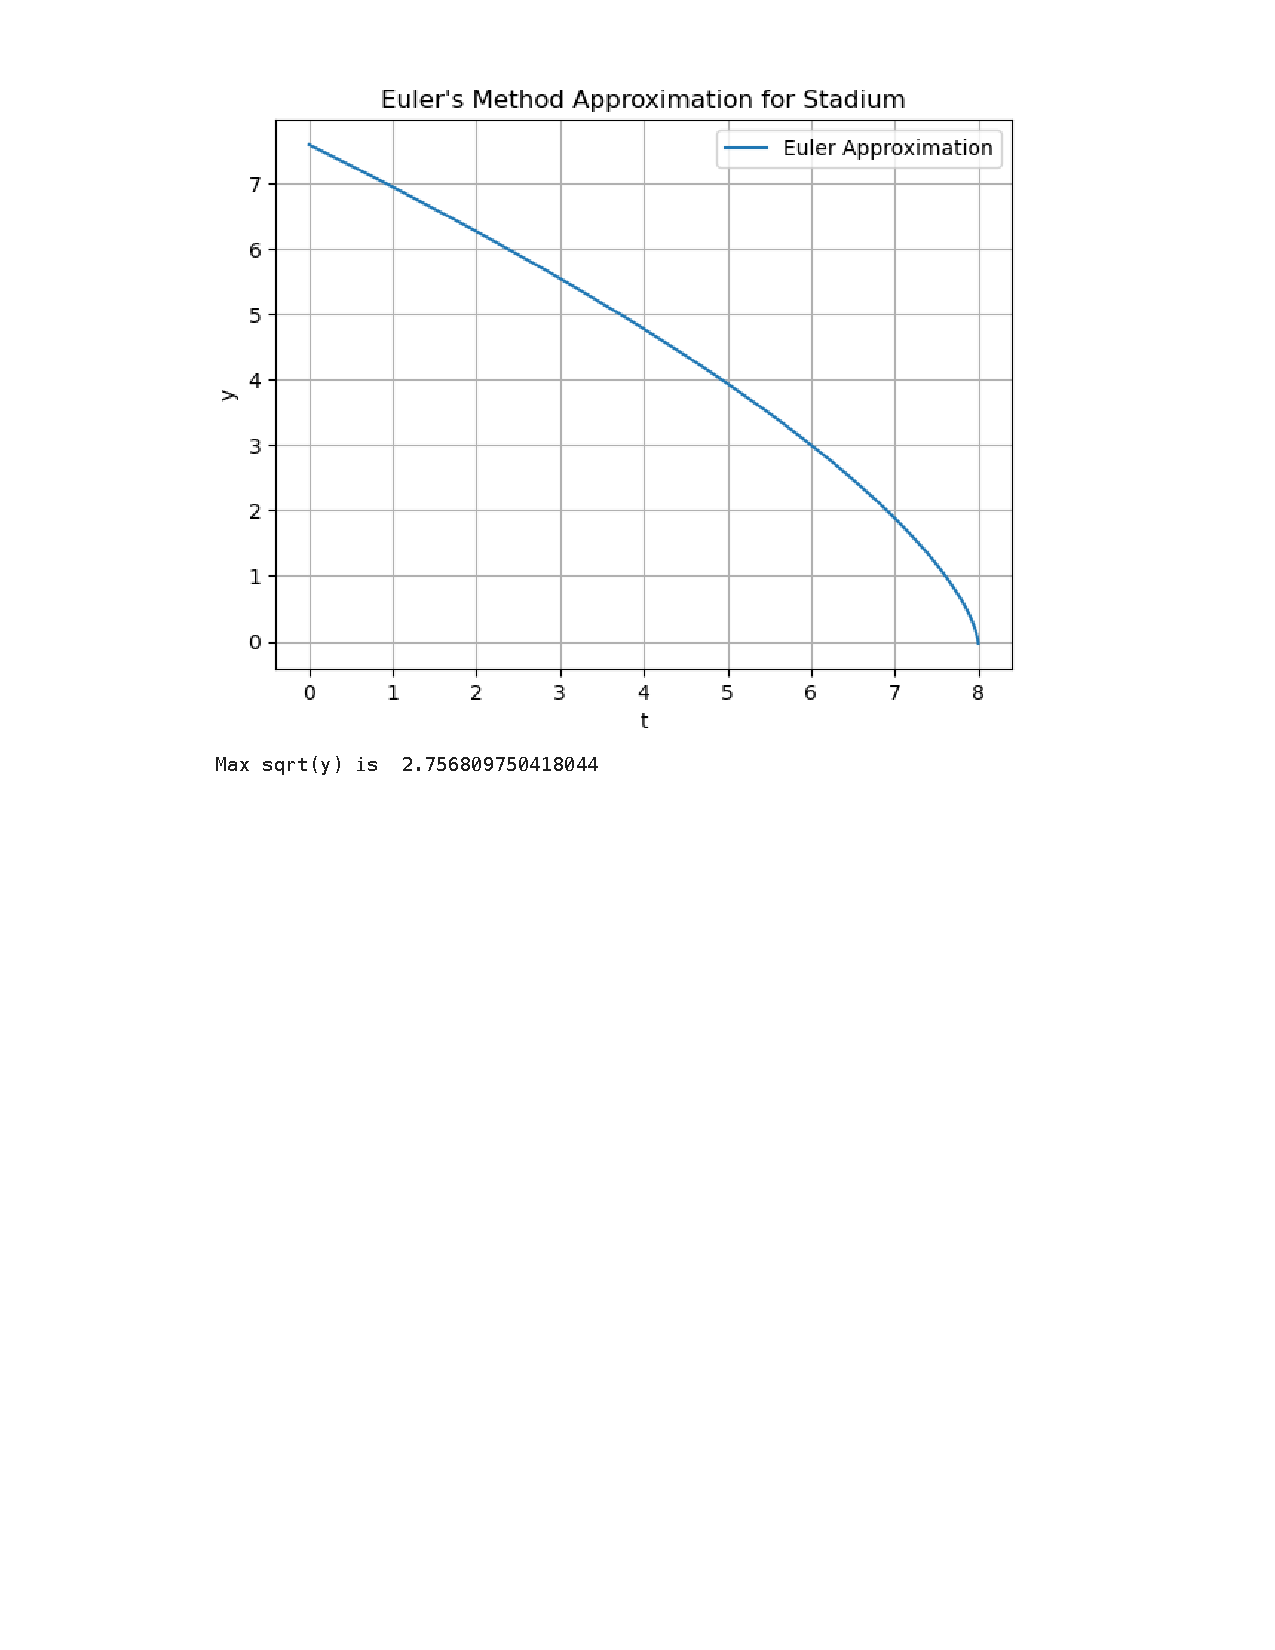
\includegraphics[width=0.4\textwidth]{python/Stadium-Euler-ipynb.pdf}


\end{slide}	
\end{solution}







\addcontentsline{toc}{subsection}{Numerical Methods for ODEs}

\addcontentsline{toc}{subsubsection}{Euler Method}
\addcontentsline{toc}{subsubsection}{Heun Method}


\begin{slide}

\question

Numerical Methods for:
\[ y' = f(t,y) \]

\SavedDefinitionRender{EulerMethod}

\SavedDefinitionRender{HeunMethod}

\end{slide}

\addcontentsline{toc}{subsubsection}{Runge-Kutta (4th order) Method}

\begin{slide}


\SavedDefinitionRender{RK4Method}


Desmos with all these three methods:
\hfil 
\url{https://www.desmos.com/calculator/haolaltd9s}


Consider the ODE $\dfrac{dy}{dx} = 2x\sin(x^2)$.
\begin{parts}
	\item Recall the meaning of the line segments in the slope field for this ODE.

	\item Consider the solution satisfying $y(0)=0$. With a step $h=0.1$, find the largest interval that the approximations stay within 0.1 distance of the exact solution.

\end{parts}

	
\end{slide}




\begin{solution}
\begin{slide}

The exact solution is 
\[
y = 1 - \cos(x^2).
\]

And by observing it on Desmos: 
\begin{center}
	\url{https://www.desmos.com/calculator/qflikqjufs}
\end{center}

We conclude that
\begin{itemize}
	\item Euler: $x< 1.2$
	\item Heun: $x < 5.6$
	\item Runge-Kutta: all $x$ ?
\end{itemize}
	
\end{slide}
	
\end{solution}



\addcontentsline{toc}{subsection}{Dimensional Analysis}

\begin{slide}

\question 

\textbf{Dimensional Analysis}

\SavedDefinitionRender{FundamentalDimensions}

\begin{parts}

\item When can we add/subtract quantities? With different dimensions? With the same dimensions?

\item When can we equate quantities? With different dimensions? With the same dimensions?

\item When can we multiply/divide quantities? With different dimensions? With the same dimensions?

\item It is convenient to define some functions as a power series (e.g. $e^x = 1 + x + \frac{x^2}{2} + \frac{x^3}{6}+ \cdots$). What condition on the dimension of $x$ is required to be able to do this?

\item What are the dimensions of a derivative $\frac{dy}{dx}$? What are the dimensions of an integral $\int y \, dx$?
	
\end{parts}

\begin{slidesonly}
	\bigskip
\end{slidesonly}


\textbf{Modelling:} Relationship between the variables in a model must be dimensionally consistent.

\end{slide}




\begin{slide}

\question \label{q:radioactive}

\paragraph{Non-Dimensionalization.}

Consider the model for a mass undergoing radioactive decay:
\[ \frac{dm}{dt} = -km \]
with $m(0) = m_0$.

\begin{parts}
	\item What are the units of $k$? What are the units of $t_c=\frac{1}{k}$? % $t_c$ is related to the half-life of the radioactive decay

	\item Introduce new variables: $\tau = \frac{t}{t_c}$ and $\overline{m}(\tau) = \frac{m(t)}{m_0}$. What is the ODE satisfied by $\overline{m}(\tau)$? What are its units? What are the parameters for this equation?
	
\end{parts}

\end{slide}




\begin{solution}
\begin{slide}

\begin{parts}
	\item The units of m are mass $M$, so the units of $\frac{dn}{dt}$ are $\frac{M}{T}$.
	
	This means that the units of $k$ must be $\frac{1}{T}$, so that $km$ matches the units on the other side of the equation.
	
	This implies that $t_c$ has the units of time $T$.
	
	\item $\displaystyle\frac{d\overline{m}}{d\tau} = \frac{1}{m_0} \frac{dm}{d\tau} = \frac{1}{m_0} \frac{dm}{dt} \frac{dt}{d\tau} = \frac{t_c}{m_0} \frac{dm}{dt}$
	
	So we get 
	\[
	\frac{d\overline{m}}{d\tau} 
		= \frac{t_c}{m_0} \frac{dm}{dt} 
		= -\frac{t_c}{m_0} k m(\tau)
		= -\frac{1}{m_0} m(\tau)
		= - \overline{m}
	\]
	and $\overline{m}(0)=1$.
	
\end{parts}
\end{slide}

\end{solution}

	







\begin{slide}
\question \label{q:budworms}
	
\begin{problem}[Spruce Budworm Outbreak]
Consider the model for spruce budworm outbreak in Eastern Canada\footnote{See ``Nonlinear Dynamics and Chaos'' by Strogatz.}.

\[
\frac{dN}{dt} = R N \left( 1 - \frac{N}{K} \right) - \frac{B N^2}{A^2 + N^2}.
\]

The first term accounts for resource-limited population growth within a tree and the second term accounts for the predation of the budworms by birds.
\end{problem}

\begin{parts}
	\item What are the units of $N, A, B, K$?
	


	\item To ``non-dimensionalize'' this ODE, what variable would you consider instead of $N$?  What ODE is satisfied by your new variable? How many parameters do you have now?
	
%	What is the ODE satisfied by $x(\tau)$?

	
\end{parts}

\end{slide}

\begin{solution}
\begin{slide}

\begin{parts}
	\item \begin{itemize}
		\item $[N] =$ budworm population ($N$)
		\item $[K] =$  carrying capacity of budworm population ($N$)
		\item $[R] =\frac{1}{T}$ 
		\item $[A] = N$
		\item $[B] = \frac{N}{T}$
 	\end{itemize}
 	
 	\item Consider the new variables\footnote{This is not the only way to do this.}:
		\begin{itemize}
			\item $x = N/A$ the non-dimensional budworm population
			\item $\tau = \frac{Bt}{A}$ the non-dimensional time
			\item $r = \frac{RA}{B}$ the non-dimensional growth rate
			\item $k = \frac{K}{A}$ the non-dimensional carrying capacity
		\end{itemize}


	\begin{align*}
		\frac{dx}{d\tau} 
			& = \frac{1}{A} \frac{dN}{dt} \frac{dt}{d\tau}
			= \frac{1}{B} R N \left( 1 - \frac{N}{K} \right) - \frac{N^2}{A^2 + N^2} \\
			& = \frac{1}{B} A R x \left( 1 - A\frac{x}{K} \right) - \frac{x^2}{(1 + x^2)} \\
			& = r x \left(1-\frac{x}{k}\right)- \frac{x^2}{(1 + x^2)}
	\end{align*}


	OR consider the new variables:
	\begin{itemize}
		\item $x = N/K$ non-dimensional budworm population (fraction of its carrying capacity)
		\item $b = B/K$ with units 1/(amount$^2 \times$ time
		\item $a = A/K$ non-dimensional
	\end{itemize}
	
	\begin{align*}
		\frac{dx}{d\tau} 
			& = \frac{1}{K} \frac{dN}{dt} \frac{dt}{d\tau}
			= R x \left( 1 - x \right) - \frac{1}{K}\frac{B N^2}{A^2 + N^2} \\
			& = R x \left( 1 - x \right) - \frac{b x^2}{a + x^2}
	\end{align*}


	
\end{parts}	
	
\end{slide}

\end{solution}	







\addcontentsline{toc}{subsubsection}{Buckingham Pi Theorem}

\begin{slide}

\question

\SavedDefinitionRender{DimensionalMatrix}

\SavedDefinitionRender{BuckinghamPiThm}
	
%	\begin{center}
%		\begin{tikzpicture}[scale=0.5]
%		  \draw[fill=brown!65!black,draw=none] (-1,0.1) rectangle (1,0);
%		  \draw (-1,0) -- (1,0);
%		  \draw[ultra thick] (0,0) -- (1,-4);
%		  \draw[thick, fill=black!20!white] (1,-4) circle (0.5) node {m};
%		%  \draw[dashed, gray] (0,0) -- (0,-4);
%		%  \draw[->,gray] (0,-3) node[above] {$\quad\theta$} arc (-90:-76:3);
%		%  \draw[->] (1, -4.75) -- (1, -5.25) node[below] {\small $\vec{F}_g$};
%		%  \draw[->] (1.1, -3.3) -- (0.95, -2.7) node[right] {\small $\vec{T}$};  
%		\end{tikzpicture}
%	\end{center}	


%\begin{minipage}{.15\textwidth}
%	\begin{center}
%		\begin{tikzpicture}[scale=0.6]
%		  \draw[fill=brown!65!black,draw=none] (-1,0.1) rectangle (1,0);
%		  \draw (-1,0) -- (1,0);
%		  \draw[ultra thick] (0,0) -- (1,-4);
%		  \draw[thick, fill=black!20!white] (1,-4) circle (0.5) node {m};
%		%  \draw[dashed, gray] (0,0) -- (0,-4);
%		%  \draw[->,gray] (0,-3) node[above] {$\quad\theta$} arc (-90:-76:3);
%		%  \draw[->] (1, -4.75) -- (1, -5.25) node[below] {\small $\vec{F}_g$};
%		%  \draw[->] (1.1, -3.3) -- (0.95, -2.7) node[right] {\small $\vec{T}$};  
%		\end{tikzpicture}
%	\end{center}	
%\end{minipage}
%	%
%\begin{minipage}{.35\textwidth}
%Consider a pendulum. We make assumptions:
%	\begin{itemize}
%		\item The pivot is frictionless
%		\item The rod is massless
%		\item Air resistance is neglected
%%		\item The gravitational field is uniform
%		\item The ceiling is infinitely rigid
%		\item $\cdots$
%	\end{itemize}
%\end{minipage}
%
%\bigskip
%\bigskip
%\bigskip

\begin{problem}
	Consider a pendulum. We make assumptions:

	\begin{minipage}{2.5in}
			\begin{itemize}
				\item The pivot is frictionless
				\item The rod is massless
				\item Air resistance is neglected
		%		\item The gravitational field is uniform
				\item The ceiling is infinitely rigid
				\item $\cdots$
			\end{itemize}		
	\end{minipage}
	\begin{minipage}{0.5in}
		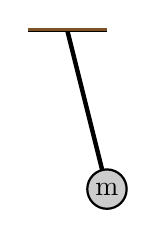
\begin{tikzpicture}[scale=0.5]
		  \draw[fill=brown!65!black,draw=none] (-1,0.1) rectangle (1,0);
		  \draw (-1,0) -- (1,0);
		  \draw[ultra thick] (0,0) -- (1,-4);
		  \draw[thick, fill=black!20!white] (1,-4) circle (0.5) node {m};
		%  \draw[dashed, gray] (0,0) -- (0,-4);
		%  \draw[->,gray] (0,-3) node[above] {$\quad\theta$} arc (-90:-76:3);
		%  \draw[->] (1, -4.75) -- (1, -5.25) node[below] {\small $\vec{F}_g$};
		%  \draw[->] (1.1, -3.3) -- (0.95, -2.7) node[right] {\small $\vec{T}$};  
		\end{tikzpicture}
	\end{minipage}	
\end{problem}


\begin{parts}
	\item What are the units of the following variables of interest?
	\begin{enumerate}
		\item Period of the swing $[P] =$ 
		\item Pendulum mass $[m]=$
		\item Pendulum rod length $[\ell]=$
		\item Gravitational acceleration $[g]=$
		\item Amplitude of the swing $[\Theta]=$
	\end{enumerate}
	

\end{parts}

\end{slide}

\begin{slide}

\begin{parts}
\setcounter{partsitem}{1}

	\item Let us create the dimensional matrix:
	\begin{itemize}
		\item One column for each variable of interest (remember the order used for later)
		\item One row for each dimension
		\item Each term contains the power of the corresponding dimension for the corresponding variable
	\end{itemize}
	
	\begin{center}
	\begin{tabular}{cccccccl}
		& $[P]$ & $[m]$ & $[\ell]$ & $[g]$ & $[\Theta]$ & \\
		& $\downarrow$ & $\downarrow$ & $\downarrow$ & $\downarrow$ & $\downarrow$ & \\
	\multirow{3}{*}{$\mathcal{D}=\left[\begin{matrix} \, \\ \,\\ \, \end{matrix}\right.$} 
		& & & & & & 
		\multirow{3}{*}{$\left.\begin{matrix} \, \\ \,\\ \, \end{matrix}\right]$}
		& $\leftarrow M$
		\\
		& & & & & & & $\leftarrow L$ \\
		& & & & & & & $\leftarrow T$
	\end{tabular}
	\end{center}
	
	\item What is the rank of this matrix?
	\item What is the dimension of the null space? %\footnote{Use the Rank-nullity theorem.}?
	\item Find a basis for the null space.

\end{parts}

\end{slide}

\begin{slide}

For each vector of the null space basis, 
\[ \mat{2\\0\\-1\\1\\0} , \mat{0\\0\\0\\0\\1} \]

Buckingham Pi Theorem states that these correspond to non-dimensional variables $\Pi_1$ and $\Pi_2$:
\[ \Pi_1 = \frac{P^2 g}{\ell} \quad \text{ and } \quad \Pi_2 = \Theta \]

and that there is a relation between them:
\[
F(\Pi_1,\Pi_2)=0 \quad \text{ or } \quad \Pi_1 = f(\Pi_2) \quad \Leftrightarrow \quad \frac{P^2 g}{\ell} = f(\Theta)
\]
which implies that
\[ 
P = \sqrt{\frac{\ell}{g}} \cdot \overline{f}(\Theta),
\]
or in other words, the fact that the \textit{period of the pendulum is proportional to the square root of its length} is a consequence of a pure dimensional analysis of the variables in the problem.


\begin{parts}
	\setcounter{partsitem}{5}
	\item Recall the ODE for the pendulum: $ \frac{d^2\theta}{dt^2} = -\frac{g}{\ell}\sin (\theta)$. Linearize\footnote{If you are not comfortable with linearization of an ODE, check exercise 61 on \url{https://raw.githubusercontent.com/siefkenj/IBLODEs/main/dist/odes.pdf}.} it near the equilibrium $\theta=0$.
	\item Solve the linearized pendulum ODE, and compare the period of the linearized model to the nonlinear one.
\end{parts}


\end{slide}





\begin{slide}

\question

\begin{problem}

Consider the flow past a sphere.

\begin{center}
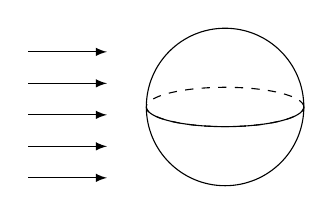
\begin{tikzpicture}
	\draw (0,0) circle (1);
	\draw[dashed] (0,0) ellipse (1cm and 0.25cm);
    \draw[variable=\t,domain=180:360,samples=100] plot ({cos(\t)},{0.25*sin(\t)});
    \foreach \i in {-0.9,-0.5,...,0.9}:
       \draw[-latex] (-2.5,{\i}) -- (-1.5,{\i});
\end{tikzpicture}
\end{center}

You don't need to know much about fluid dynamics to be able to deduce some properties of the flow. \\

The sphere is in a fluid (water) and we measure the force necessary to keep the sphere from moving downstream.

We want to understand how the drag force depends on the upstream velocity.
\end{problem}

\begin{parts}
	\item What are the units of the variables of interest\footnote{This choice is part of the modelling process.}?
	\begin{enumerate}
		\item drag force $[F]=$
		\item upstream velocity $[v]=$
		\item fluid density $[\rho]=$
		\item sphere diameter $[D]=$
		\item fluid viscosity\footnote{Fluid viscosity is the sphere's resistance to deformation by shear stress. To help with the units, the formula for the Force from viscosity is $F =\mu \cdot A \cdot u/y$, where $A$ is area, $u$ is velocity and $y$ is position.} $[\mu]= $
	\end{enumerate}
	\item Create a dimension matrix $\mathcal{D}$.
	\item What is its rank? What is the dimension of its null space? Find a basis for its null space.
	\item What are the non-dimensional variables $\Pi$'s from Buckingham Pi Theorem?
	\item What relations do you obtain?
		
\end{parts}
	
\end{slide}


\begin{solution}
\begin{slide}

Solution:

\[ \mathcal{D} = 
	\mat{1 & 0 & 1  & 0 & 1 \\
		1 & 1 & -3 & 1 & -1 \\
		-2 & -1 & 0 & 0 & -1}
\]
for rows $M,L,T$.

Its rank is 3, so there are 2 independent null vectors:
\[ \mat{0\\1\\1\\1\\-1} \quad \text{ and } \quad \mat{1\\-2\\-1\\-2\\0}
\]
corresponding to
\[
\Pi_1 = \frac{\rho v D}{\mu}
\quad \text{ and } \quad 
\Pi_2 = \frac{F}{\frac12\rho v^2 D^2}
\]

\begin{itemize}
	\item $\Pi_1 = $ Reynolds number (Re) which determines the relation between inertia and viscous forces in a fluid flow.
	\item $\Pi_2 = $ is the drag coefficient ($C_d$)
\end{itemize}

So dimensional analysis reveals:
\[ \Pi_2 = f(\Pi_1) \]
which means that the drag coefficient depends on the fluid's Reynolds number. \\

\hrule

Could have also obtained
\[ \mat{0\\1\\1\\1\\-1} \quad \text{ and } \quad \mat{1\\0\\1\\0\\-2} \]
which gives a different $\Pi_2$ and a different relation.
\end{slide}


\begin{slide}

	Using python to find the null space gives yet another set of different $\Pi_1$ and $\Pi_2$.

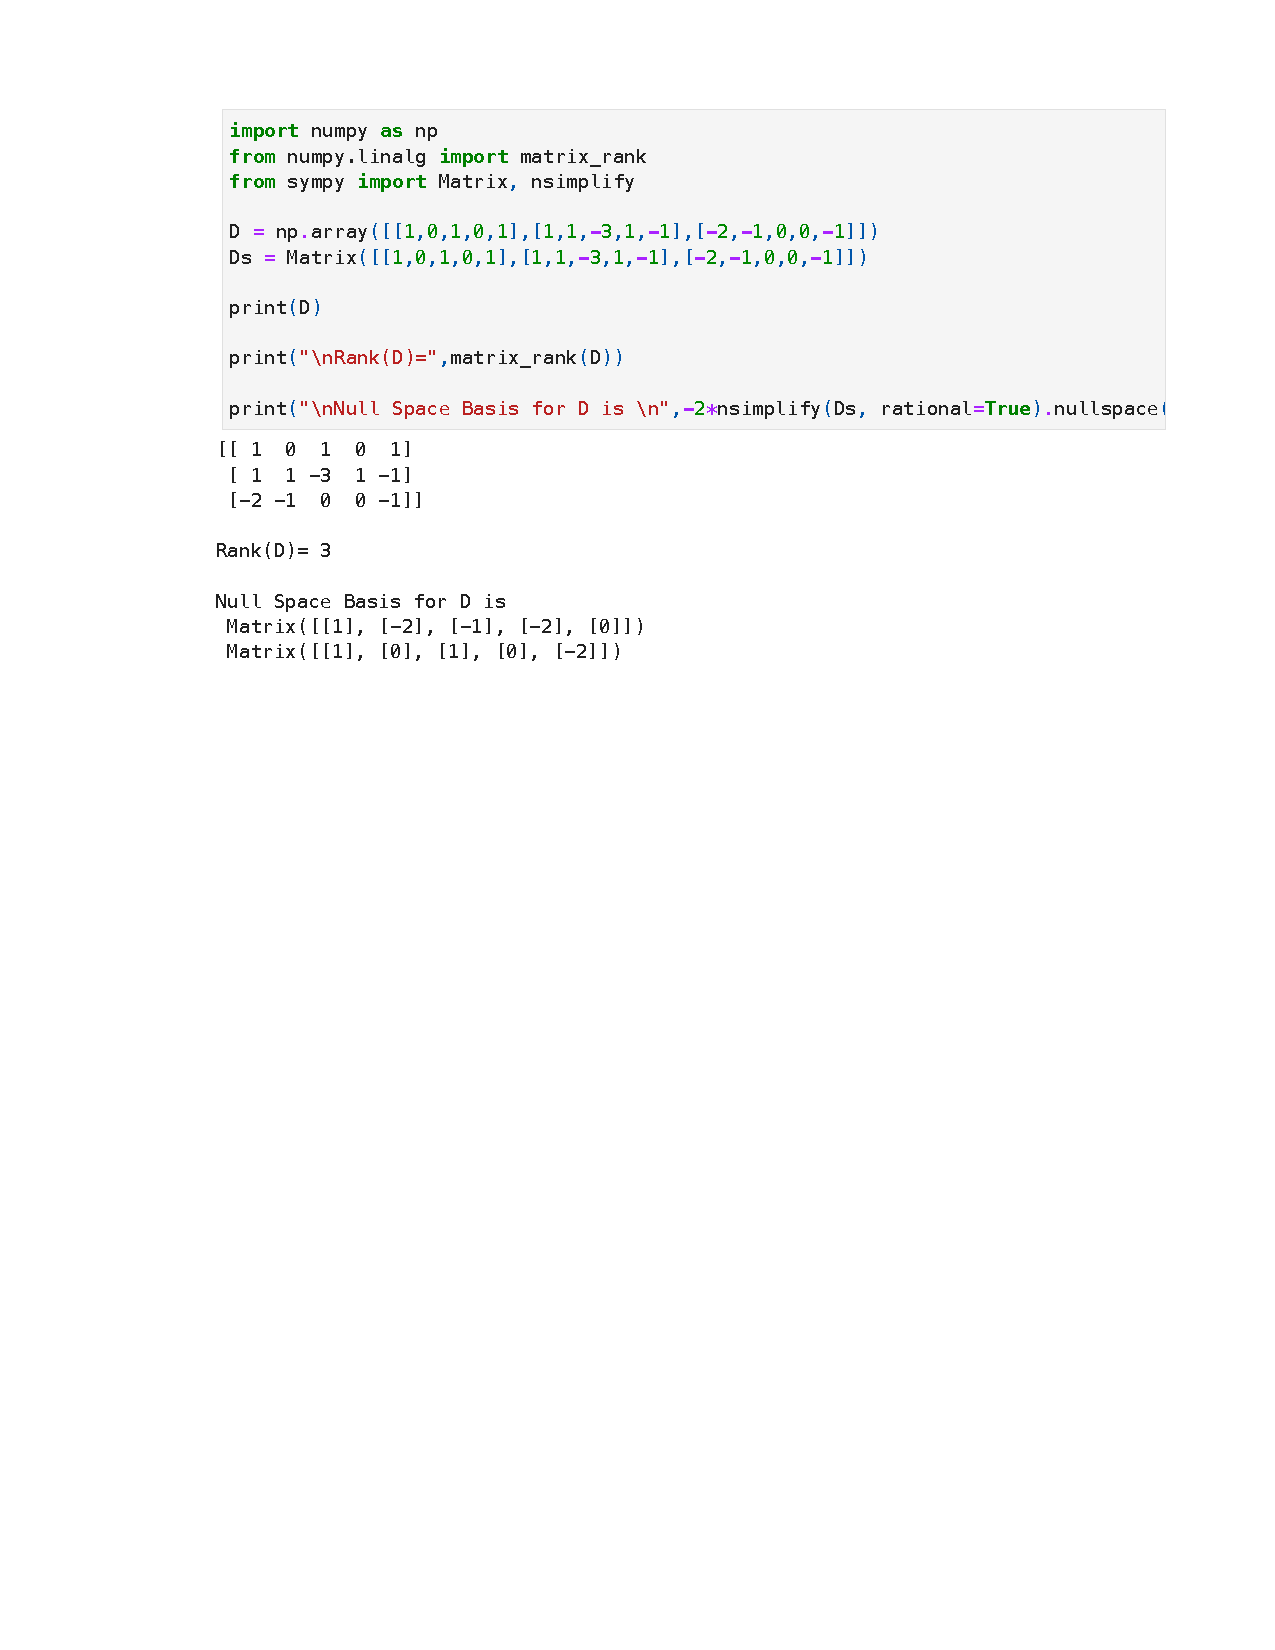
\includegraphics[width=0.75\textwidth]{python/sphere-dimensionanalysis.pdf}

	
\end{slide}
\end{solution}


\begin{slide}

\question

\begin{parts}
	\item Use Buckingham Pi Theorem on Exercise \ref{q:radioactive} about radioactive decay.
	\item Use Buckingham Pi Theorem on Exercise \ref{q:budworms} about the budworm population.
\end{parts}
	
\end{slide}





%
%\begin{slide}
%
%\question
%
%\begin{problem}[Dog Shampoo]
%Scientists are testing the effect of different dog shampoos. Let
%\begin{itemize}
%	\item $F = $ number of fleas (in millions)
%	\item $D = $ number of dogs (in thousands)
%	\item $a = $ effect of different dog shampoos
%\end{itemize}
%and consider the model: % for the interaction between them:
%\begin{align*}
%	F' & = -(1+a)F + D - 2 \\
%	D' & = -2F + (1-a)D + 1
%\end{align*}
%
%which is based on the following premises:
%\begin{itemize}
%	\item[(P1$_F$)] Ignoring all else, the number of parasites decays in proportion to its population (with constant $1+a$).
%	\item[(P2$_F$)] Ignoring all else, parasite numbers grow in proportion to the number of hosts (with constant 1).
%	\item[(P1$_D$)] Ignoring all else, hosts numbers grow in proportion to their current number (with constant $1-a$).
%	\item[(P2$_D$)] Ignoring all else, host numbers decrease in proportion to the number of parasites (with constant 2).
%	\item[(P1$_C$)] Anti-flea collars remove 2 million fleas per year.
%	\item[(P2$_C$)] Constant dog breeding adds 1 thousand dogs per year.
%\end{itemize}
%\end{problem}
%
%\begin{parts}
%	\item How are the premises expressed in the differential equations?
%	\item Find the equilibrium solutions for each value of $-1 \leq a \leq $.
%	\item Use \href{https://utoronto.syzygy.ca/jupyter/user-redirect/git-pull?repo=https://github.com/bigfatbernie/IBLMathModeling&subPath=book/python/fleas_dogs.ipynb}{\tt fleas_dogs.ipynb} and eigenvalues to check the stability\footnote{If you are not comfortable with studying the stability of the equilibrium solutions of a system of ODEs, then check exercises 32--61 of the same textbook. You can also check sections 2.4 and 2.5 of the textbook \href{https://raw.githubusercontent.com/siefkenj/IBLODEs/main/diffyqs-by-jiri-lebl/diffyqs.pdf}{\tt ``Diffy Qs'' by Jiri Lebl}.} of the equilibrium points for different values of $-1 \leq a \leq 1$.
%\end{parts}
%
%
%
%
%\end{slide}




\addcontentsline{toc}{subsection}{Modelling with Systems of ODEs}


\begin{slide}

\question

\begin{problem}[Dog Shampoo]\label{flea_dog}
Scientists are testing the effect of different dog shampoos. Let
\begin{itemize}
	\item $F = $ number of fleas (in millions)
	\item $D = $ number of dogs (in thousands)
	\item $a = $ effect of different dog shampoos
\end{itemize}
and consider the model: % for the interaction between them:
\begin{align*}
	F' & = -(1+a)F + D - 2 \\
	D' & = -2F + (1-a)D + 1
\end{align*}

which is based on the following premises:
\begin{itemize}
	\item[(P1$_F$)] Ignoring all else, the number of parasites decays in proportion to its population (with constant $1+a$).
	\item[(P2$_F$)] Ignoring all else, parasite numbers grow in proportion to the number of hosts (with constant 1).
\begin{slidesonly}
	\vspace{3cm}
\end{slidesonly}
	\item[(P1$_D$)] Ignoring all else, hosts numbers grow in proportion to their current number (with constant $1-a$).
	\item[(P2$_D$)] Ignoring all else, host numbers decrease in proportion to the number of parasites (with constant 2).
	\item[(P1$_C$)] Anti-flea collars remove 2 million fleas per year.
	\item[(P2$_C$)] Constant dog breeding adds 1 thousand dogs per year.
\end{itemize}
\end{problem}

\begin{parts}
	\item How are the premises expressed in the differential equations?
	\item Find the equilibrium solutions for each value of $-1 \leq a \leq 1$.
	\item Use \href{https://utoronto.syzygy.ca/jupyter/user-redirect/git-pull?repo=https://github.com/bigfatbernie/IBLMathModeling&subPath=book/python/fleas_dogs.ipynb}{\tt fleas_dogs.ipynb} and eigenvalues to check the stability\footnote{If you are not comfortable with studying the stability of the equilibrium solutions of a system of ODEs, then check exercises 32--61 of the \href{https://raw.githubusercontent.com/siefkenj/IBLODEs/main/dist/odes.pdf}{\texttt{MAT244 in-class exercises}}. You can also check sections 2.4 and 2.5 of the textbook \href{https://raw.githubusercontent.com/siefkenj/IBLODEs/main/diffyqs-by-jiri-lebl/diffyqs.pdf}{\texttt{``Diffy Qs'' by Jiri Lebl}.}} of the equilibrium points for different values of $-1 \leq a \leq 1$.
\end{parts}




\end{slide}






\addcontentsline{toc}{subsubsection}{Linearization of ODEs}


\begin{slide}

\question

\begin{problem}[Mammalian Circadian Clock]\label{circadian}

\begin{center}
 \begin{tikzpicture}[scale=0.65]
 
        % Setup the style for the states
        \tikzset{node style/.style={state, 
                                    minimum width=1.0cm,
                                    line width=0.5mm,
                                    fill=gray!20!white}}
        % Draw the states
        \node[draw,line width=0.5mm,fill=gray!20!white] at (0, 0)     (eb)     {E-Box};
        \node[node style] at (5, 2)     (mn)     {mRNA};
        \node[node style] at (5, 5.5)     (mc)     {mRNA};
        \node[node style] at (0, 5.5)     (pc)     {\textbf{PER}};
        \node[node style] at (0, 2)     (pn)     {PER};

        \draw[dashed] (-1,4.3) -- (6,4.3);
%        \draw[thick] (-1,-0.4) -- (0.8,-0.4) -- (0.8, 0.3) -- (1.8,0.3);
        % Connect the states with arrows
        \draw[every loop,
              auto=right,
              line width=0.5mm,
              >=latex,
              draw=black,
              fill=black]
            (eb) edge[bend left=10] node {transcription} (mn)
            (mn) edge[] node {nuclear export} (mc)
            (mc) edge[] node {translation} (pc)
            (pc) edge[] node {nuclear import} (pn)
            (pn) edge[] node {inhibition} (eb);
    \end{tikzpicture}
%    \caption{A diagram of the transcription-translation feedback loop of the mammalian circadian clock. When the enhancer-box (E-Box) on the DNA is active, messenger RNA (mRNA) is produced. The mRNA is exported from the nucleus where it is translated into PER protein. The protein is imported into the nucleus where it inhibits the the E-Box. \label{fig:circadianTTFL}}
\end{center}

When the enhancer-box (E-Box) on the DNA is active, messenger RNA (mRNA) is produced. The mRNA is exported from the nucleus where it is translated into PER protein. The protein is imported into the nucleus where it inhibits the E-Box. It is the cytosolic concentration of PER (highlighted) that indicates the time of day.

\begin{slidesonly}
	\vspace{2cm}
\end{slidesonly}

We get the model:
\begin{itemize}
	\item $x_1 = $ enhancer box on the DNA (E-box)
	\item $x_2, x_3 = $ mRNA inside/outside the nucleus
%	\item $x_3 = $ mRNA outside the nucleus
	\item $x_4, x_5 = $ PER outside/inside the nucleus
%	\item $x_5 = $ PER inside the nucleus
\end{itemize}
We get:

\hfil \begin{minipage}{.4\textwidth}
\begin{align*}
	x_1' & = -x_1 + e^{-\alpha x_5} \\
	x_2' & = -x_2 + x_1 \\
	x_3' & = -x_3+ x_2 
\end{align*}	
\end{minipage}
\quad 
\begin{minipage}{.4\textwidth}
\begin{align*}
	x_4' & = -x_4 + x_3 \\
	x_5' & = -x_5+ x_4 
\end{align*}	
\end{minipage}

where the exponential term represents the fact that the PER protein inhibits the E-box with ``strength'' $\alpha$.
\end{problem}

\begin{parts}
	\item Find an approximation for the equilibrium solution for $\alpha = 1$.
	\item This is a nonlinear problem. To linearize\footnote{If you are not comfortable with linearization of a system of ODEs, check exercise 61 on \url{https://raw.githubusercontent.com/siefkenj/IBLODEs/main/dist/odes.pdf}.} it around an equilibrium solution, find the Jacobian (or total derivative) $J$.
	\item Use \href{https://utoronto.syzygy.ca/jupyter/user-redirect/git-pull?repo=https://github.com/bigfatbernie/IBLMathModeling&subPath=book/python/circadian.ipynb}{\tt circadian.ipynb} and eigenvalues to check the stability of the equilibrium points for different values of $\alpha \in [0,100]$.
\end{parts}

%
%\paragraph{TO DO:} CREATE python that takes alpha and computes the jacobian matrix, its eigenvalues and graphs the real part of the eigenvalues as a function of alpha.



\end{slide}


\begin{solution}

\begin{slide}

\begin{parts}
	\item We get: $x_1 = x_2 = x_3 = x_4 = x_5$ and
	\[ x_5 = e^{-\alpha x_5} \]
	
	We have to approximate the solutions to this equation, e.g. using Newton's method.
	
	\item The Jacobian is:
		\[ J = 
			\mat { 	-1 & 0 & 0 & 0 & -\alpha e^{-\alpha x_5} \\
					1 & -1 & 0 & 0 & 0 \\
					0 & 1 & -1 & 0 &  0 \\
					0 & 0 & 1 & -1 &  0 \\
					0 & 0 & 0 & 1 & -1 
					}
		\]	
	\item The solutions are in \href{https://utoronto.syzygy.ca/jupyter/user-redirect/git-pull?repo=https://github.com/bigfatbernie/IBLMathModeling&subPath=book/python/circadian.ipynb}{\tt circadian5-sol.ipynb}.
	
	Basically we need to find the (5) eigenvalues for each value of $\alpha \in [0,100]$ and check when:
	\begin{itemize}
		\item All negative $\Rightarrow $ stable equilibrium
		\item One positive $\Rightarrow $ unstable equilibrium
	\end{itemize}
	
	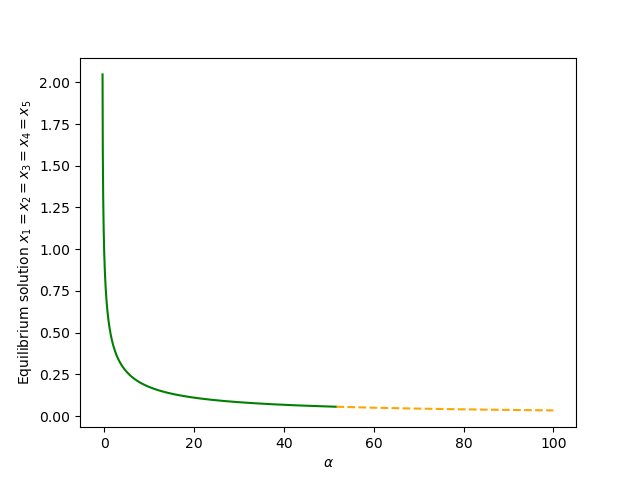
\includegraphics[width=200pt]{images/circadian5.png}
	
	
	Observe that in this case, we are actually looking for the \textbf{unstable} regime, when periodic solutions appear -- check the last part of the \texttt{Jupyter Notebook}. These only appear when the feedback in strong enough.
\end{parts}
	
\end{slide}	
\end{solution}



\addcontentsline{toc}{subsection}{ODE Bifurcations}


\begin{slide}
\question

From the previous question, we obtained equilibrium solutions that changed from stable to unstable as we changed the parameter $\alpha$ -- see the graph below.
	\begin{center}
		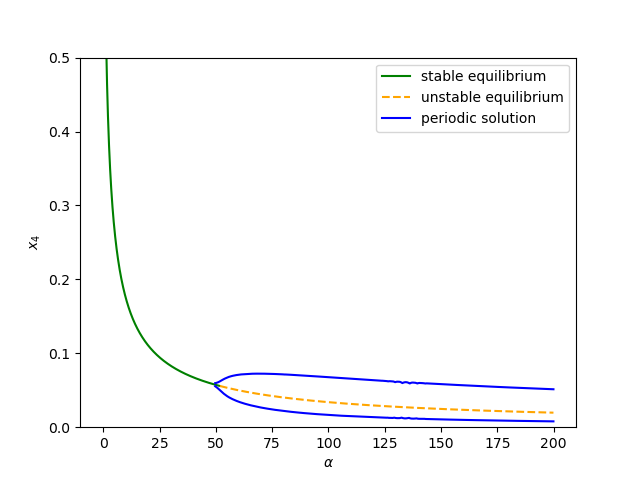
\includegraphics[width=225pt]{images/circadian5-periodic.png}
	\end{center}

This is called a \textbf{bifurcation}. \\

%\bigskip

Another type of bifurcation involves the creation of disappearance of equilibria as a parameter changes.

There are several typical types of bifurcations.

\end{slide}


\begin{slide}

\SavedDefinitionRender{bifurcations}

Decide on the type of bifurcation for each ODE.

\begin{parts}
	\item The ODE from Exercise \ref{flea_dog}.
	\item The system of ODEs from Exercise \ref{circadian}.
	\item The ODE $\frac{dx}{dt} = rx - x^2$.
	\item The ODE $\frac{dx}{dt} = r + x^2$.
	\item The ODE $\frac{dx}{dt} = rx - x^3$.
	\item The following system of ODEs as $\mu$ changes: \\
	$ \begin{cases}
 		\frac{dx}{dt} & = \mu x -  \omega y \\[5pt]
 		\frac{dy}{dt} & = \omega x + \mu y
	\end{cases}
	$
	\item The Lotka-Volterra model for $0< a < 1$: \\
	$ \begin{cases}
 		\frac{dx}{dt} & = a xy - x - 2 + \frac1a\\[5pt]
 		\frac{dy}{dt} & = y - \frac12 xy - 2 + \frac1a
	\end{cases}
	$
\end{parts}
	
	
\end{slide}


\begin{solution}
\begin{slide}
\begin{parts}
	\item Change of stability bifurcation
	\item Hopf bifurcation
	\item Transcritical bifurcation: $x(r-x) = 0$ so $x=0$ and $x=r$ are equilibria and they swap stability at $r=0$.
	\item Saddle-node bifurcation: equilibria only exist for $r<0$, one stable and one unstable.
	\item Pitchfork bifurcation: $x(r-x^2)=0$ implies
	\begin{itemize}
		\item $r\leq 0$: equilibria at $x=0$
		\item $r>0$: equilibria at $x=0$ and $x=\pm \sqrt{r}$
	\end{itemize}
	See \url{https://www.desmos.com/calculator/uksexnwbdz} about pitchfork perturbation.
	\item Hopf bifurcation: Equilibrium at $(0,0)$ and with eigenvalues $\mu \pm \omega i$, so
	\begin{itemize}
		\item $\mu<0$: stable spiral
		\item $\mu = 0$: stable centre (periodic orbit)
		\item $\mu > 0$: unstable spiral
	\end{itemize}
	\item Equilibrium at $(\frac{1}{a},2)$ and
	\begin{itemize}
		\item $a < 1-\frac{\sqrt{3}}{2} \approx 0.134$: two negative eigenvalues (stable)
		\item $1-\frac{\sqrt{3}}{2}< a < \frac12$: stable spiral
		\item $ a = \frac12$: stable centre (periodic orbit)
		\item $ a > \frac12$: unstable spiral
	\end{itemize}
	
	Change in qualitative behaviour at $a = 1-\frac{\sqrt{3}}{2}$ and Hopf at $a = \frac12$.
	
	Calculations at \href{https://utoronto.syzygy.ca/jupyter/user-redirect/git-pull?repo=https://github.com/bigfatbernie/IBLMathModeling&subPath=book/python/bifurcation-LotkaVolterra.ipynb}{\tt bifurcation-LotkaVolterra.ipynb}.
	
	Visualize also here \url{https://www.desmos.com/calculator/aydzcpccy4}

\end{parts}
	
\end{slide}
	
\end{solution}








\addcontentsline{toc}{subsection}{Modelling with PDEs}

\begin{slide}
\question \label{transport}

\begin{problem}[Transport Equation]
	
Consider a river with the water moving at speed $v$.
\begin{center}
\includegraphics*[width=175pt]{images/river.pdf}
\end{center}

We want to model $w(x,t)$, the density of pollutant in the river at the point $x$ and time $t$.
\end{problem}

\begin{parts}
\item How much pollutant is there in $[a,b]$?
\item How does pollutant change in $[a,b]$?
\item Find a ``conservation of pollutant'' equation.
\item Simplify the equation to obtain a PDE for $w(x,t)$.

\textit{Hint: Recall the FTC: $f(b)-f(a) = \int_a^b f'(x) dx$.}

\end{parts}


\end{slide}


\begin{solution}
\begin{slide}

\begin{parts}
	\item $\displaystyle T(t) = R \int_a^b w(x,t) ~dx$	, 	where $R$ is the width of the river.
	\item Pollutant goes in through the left and out through the right, so the change in the amount of pollutant is
	\[
	w(a,t) v R - w(b,t) v R = v R \bigskip(w(a,t) - w(b,t)\big).
	\]

	\item Because pollutant is neither created or destroyed, we know that:
	\[T'(t) = v R \bigskip(w(a,t) - w(b,t)\big) \]
	
	\begin{slidesonly}
	\vspace{3cm}
	\end{slidesonly}	
	
	\item \hfil \\[-35pt]
	\begin{align*}
		R \int_a^b \frac{\partial w}{ \partial t} (x,t) \, dx & = v R \bigskip(w(a,t) - w(b,t)\big) \\
		\int_a^b \frac{\partial w}{ \partial t} (x,t) ~dx & = v \bigskip(w(a,t) - w(b,t)\big) \\
		\int_a^b \frac{\partial w}{ \partial t} (x,t) ~dx & = -v \int_a^b \frac{\partial w}{\partial x} (x,t) ~dx
	\end{align*}
	\[
	\int_a^b \frac{\partial w}{ \partial t} + v \frac{\partial w}{ \partial x} ~dx = 0
	\]
	
	Because $a,b$ are arbitrary points in the river, we can conclude that
	\[ 
	\frac{\partial w}{ \partial t} + v \frac{\partial w}{ \partial x} = 0
	\qquad \text{ or } \qquad 
	w_t + v \cdot w_x = 0
	\]
	
\end{parts}

	Here is a Jupyter notebook with the Lax-Friedrichs Method approximation for the transport equation:
	\begin{itemize}
		\item \href{https://utoronto.syzygy.ca/jupyter/user-redirect/git-pull?repo=https://github.com/bigfatbernie/IBLMathModeling&subPath=book/python/transport_LaxFriedrichs.ipynb}{\tt transport\_LaxFriedrichs.ipynb}
	\end{itemize}
	
\end{slide}
	
\end{solution}


\addcontentsline{toc}{subsubsection}{Method of Characteristics}


\begin{slide}
\question

\SavedDefinitionRender{characteristics}
	
\begin{parts}

	\item Find the solution of the transport equation from Exercise \ref{transport} using the Method of Characteristics with the initial condition $u(x,0) = p(x)$.
	
	\item Find the solution of the same problem with an accelerating river: $v = 3t^2$.
	
	\item Find the solution for $w_t + 5 w_x = 2$.

	\item Find the solution for $w_t + 3t^2 w_x = 2$.

	\item Find the solution for $w_t + 3t^2 w_x = -x$.
	
\end{parts}

\begin{center}
	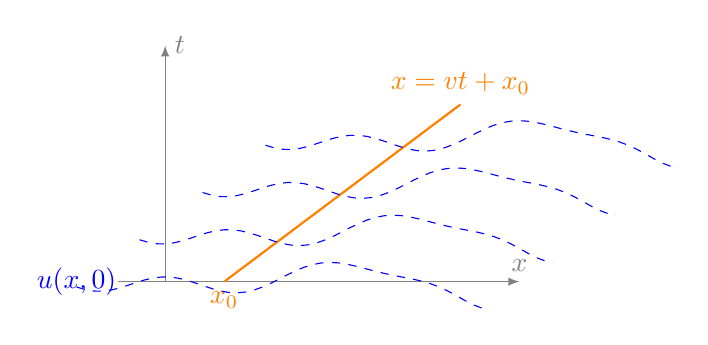
\begin{tikzpicture}[scale=1.5]
		\draw[gray] (-0.4,0)--(0,0);
		\draw[latex-latex, gray] (3,0) node[above] {$x$} -- (0,0) -- (0,2) node[right] {$t$};
		\draw[orange, thick] (0.5,0) node[below] {$x_0$} -- (2.5,1.5) node[above] {$x=vt+x_0$};
		\foreach \i in {0,0.4,0.8,1.2}:
			\draw[dashed, blue,variable=\x,domain=-0.75:2.75,samples=50] plot ({\x+4*\i/3},{sin(\x*180)*(-1.2*\x*\x*\x*\x+3.7*\x*\x*\x-5.8*\x)/20+0.04+\i});
		\draw[blue] (-0.75,0) node {$u(x,0)$};
	\end{tikzpicture}
	\end{center}	
	
	

\end{slide}
%
%
%\begin{slide}
%
%\begin{center}
%	\begin{tikzpicture}[scale=1.5]
%		\draw[gray] (-0.4,0)--(0,0);
%		\draw[latex-latex, gray] (3,0) node[above] {$x$} -- (0,0) -- (0,2) node[right] {$t$};
%		\draw[orange, thick] (0.5,0) node[below] {$x_0$} -- (2.5,1.5) node[above] {$x=vt+x_0$};
%		\foreach \i in {0,0.4,0.8,1.2}:
%			\draw[dashed, blue,variable=\x,domain=-0.75:2.75,samples=50] plot ({\x+4*\i/3},{sin(\x*180)*(-1.2*\x*\x*\x*\x+3.7*\x*\x*\x-5.8*\x)/20+0.04+\i});
%		\draw[blue] (-0.75,0) node {$u(x,0)$};
%	\end{tikzpicture}
%	\end{center}	
%\end{slide}


\begin{solution}

\begin{slide}
\begin{parts}

	\item We need to solve
	
	\begin{itemize}
		\item $	\frac{dx}{dt} = v \quad \to$  an observer moving along the river at the same speed as the river
		\item $ \frac{du}{dt} = 0 \quad \to $ for such an observer looking at the river, the pollutant density doesn't change
	\end{itemize}

		\[
	\begin{cases}
		x = vt + x_0 \\
		u\big(x(t),t\big) = C
	\end{cases}
	\]
	
	This means that when $t=0$, we get $u(x_0,0) = C = p(x_0)$, and $x_0 = x - vt$, so
	\[
	u(x,t) = C = p(x_0) = p(x-vt).
	\]
	
	The idea in a graph:
	\begin{center}
	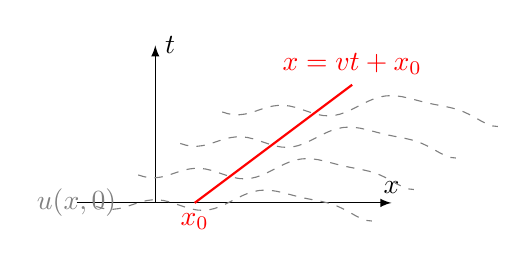
\begin{tikzpicture}
		\draw (-1,0)--(0,0);
		\draw[latex-latex] (3,0) node[above] {$x$} -- (0,0) -- (0,2) node[right] {$t$};
		\draw[red, thick] (0.5,0) node[below] {$x_0$} -- (2.5,1.5) node[above] {$x=vt+x_0$};
%		\draw[red, thick] (0.5,0) node[below] {$x_0$} -- node[above, rotate=37] {$x=vt+x_0$}(2.5,1.5);
		\foreach \i in {0,0.4,0.8,1.2}:
			\draw[dashed, gray,variable=\x,domain=-0.75:2.75,samples=50] plot ({\x+4*\i/3},{sin(\x*180)*(-1.2*\x*\x*\x*\x+3.7*\x*\x*\x-5.8*\x)/20+0.04+\i});
		\draw[gray] (-1,0) node {$u(x,0)$};
	\end{tikzpicture}
	\end{center}

	Here we can run an approximation for a specific $u(x,0)$ and $v = -1.2$: 
	\begin{itemize}
		\item \href{https://utoronto.syzygy.ca/jupyter/user-redirect/git-pull?repo=https://github.com/bigfatbernie/IBLMathModeling&subPath=book/python/transport_LaxFriedrichs.ipynb}{\tt transport\_LaxFriedrichs.ipynb}
	\end{itemize}

	\item The idea is similar but we get 
	
			\[
	\begin{cases}
		x = t^3 + x_0 \\
		u\big(x(t),t\big) = C
	\end{cases}
	\]
	
	This means that when $t=0$, we get $u(x_0,0) = C = p(x_0)$, and $x_0 = x - t^3$, so
	\[
	u(x,t) = C = p(x_0) = p(x-t^3).
	\]

		
\end{parts}

\end{slide}
	
\end{solution}




\addcontentsline{toc}{subsubsection}{Traffic Flow Model}


\begin{slide}

\question

\begin{problem}[Traffic Flow]
\begin{center}
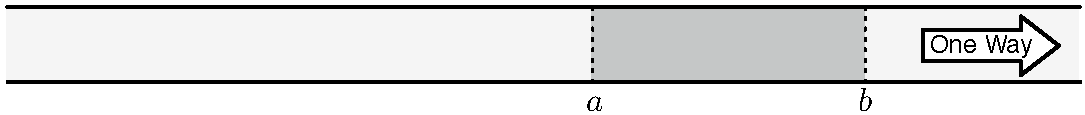
\includegraphics[width=0.9\textwidth]{images/road-long.pdf}
\end{center}
We want to model how traffic flows on a one way road.
\end{problem}

Let
\begin{itemize}
\item $\rho(x,t) = $ density of cars (number of cars per $km$) %at position $x$ and time $t$;
\item $\phi(x,t) = $ number of cars passing the point $x$ per hour % at time $t$ 
			% $=$ flux of cars.
\end{itemize}

And assume:
\begin{itemize}
	\item[(C)] Cars are conserved (they are not destroyed nor created on the road)
\end{itemize}

\begin{parts}
\item What is the total number of cars in the section of the road $x \in [a,b]$ at time $t$?

\item How does the total number of cars change in $[a,b]$?


\item Obtain an equation relating $\rho(x,t)$ and $\phi(x,t)$. The equation should not include $a$ or $b$.	

\end{parts}


\end{slide}



\begin{slide}


We need to model how fast cars move on the road: $\phi(x,t)$.

Below we graphed measurements for density and speed at the highway 401\footnote{Data from the paper \href{https://doi.org/10.1287/trsc.1090.0297}{``Calibrating Steady-State Traffic Stream and Car-Following Models Using Loop Detector Data'' by H Rakha and M Arafeh}} together with three different models to fit the data.
\begin{center}
\begin{tikzpicture}[scale=0.8]
    \begin{axis}[
            width=10cm, height=5cm, %, width=15cm, height=8cm,     % size of the image
            grid = major,
            grid style={dashed, gray!30},
            xmin=0,xmax=60,ymin=0,ymax=120,
%			minor y tick num=5,
			ytick distance = 20,
            ylabel=speed $v$ (km/h),
            xlabel=density $\rho$ (vehicles/km),
            clip mode=individual % so that the fits go on top of the data
         ]
        \addplot[only marks] table  {images/densityspeed.dat};
        \addplot[domain=0:60, very thick, samples=121, color=blue]{121.2613*(1-x/63.6628)}; % Greenshields
        \addplot[domain=0:60, very thick, samples=121, color=orange]{106.6081*(1-exp(-56.1848*(1/x-1/56.5544)))}; % Newell
        \addplot[domain=0:60, very thick, samples=121, color={black!60!green}]{109.7737/(1+exp(0.1297*(x-32.2037)))}; % logistic
    \end{axis}
\end{tikzpicture}
\end{center}

It shows three models:
\begin{itemize}
	\item[\textcolor{blue}{\textbullet}] \textcolor{blue}{Greenshields model} (linear fit of the data): $v(\rho) = v_{\max} \left(1 - \dfrac{\rho}{\rho_{\max}}\right)$
	\item[\textcolor{orange}{\textbullet}] \textcolor{orange}{Newel model}
	\item[\textcolor{black!60!green}{\textbullet}] \textcolor{black!60!green}{Logistic model}: $v(\rho) = v_{\max} / \left(1+ e^{-k(\rho - \rho_0)}\right)$
\end{itemize}

\begin{parts}
\setcounter{partsitem}{3}
	\item Using the Greenshields model, find an expression for $\phi(x,t)$.	
	\item Obtain a PDE for $\rho(x,t)$.
\end{parts}

	
\end{slide}


\begin{solution}
\begin{slide}

\begin{parts}
	
	\item $\displaystyle C(t) = \int_a^b \rho(x,t) ~dx$
	\item $\displaystyle C'(t) = \phi(a,t) - \phi(b,t)$
	\item From the previous two parts, we get
	\[ 
		\int_a^b \rho_t ~dx = \phi(a,t) - \phi(b,t)
	\]

	By using the FTC, we have $\displaystyle \phi(b,t) - \phi(a,t) = \int_a^b \phi_x(x,t) ~dx$, so we conclude that
	\[ 
		\int_a^b \rho_t + \phi_x(x,t) ~dx = 0
	\]
	Because this integral must be true for any values of $a,b$, we conclude that the integrand must be zero:
	\[ 
		\rho_t + \phi_x(x,t) = 0
	\]	
	
	
	\item $\phi(x,t) = \rho v(\rho)$
	\item We can expand the equation we found before:
	\begin{align*}
		\rho_t + \phi_x(x,t) & = 0 \\
		\rho_t + \rho_x v_{\max} \left(1 - \dfrac{\rho}{\rho_{\max}}\right) - \rho v_{\max} \dfrac{\rho_x}{\rho_{\max}} & = 0 \\
		\rho_t + \rho_x v_{\max} \left(1 - \dfrac{2 \rho}{\rho_{\max}}\right) & = 0
	\end{align*}

\end{parts}
	
\end{slide}
	
\end{solution}





\begin{slide}
\question

Let us study two interesting cases.

\begin{parts}
\item[]
\begin{center}
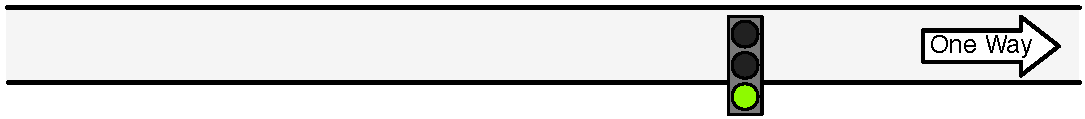
\includegraphics[width=.6\textwidth]{images/road-green.pdf}	
\end{center}


\item What is the initial car density $\rho(x,0) = \rho_0(x)$ on a one way road with a traffic light that just turned from \textbf{\textcolor{red}{red}} to \textbf{\textcolor{green}{green}}?


\begin{center}
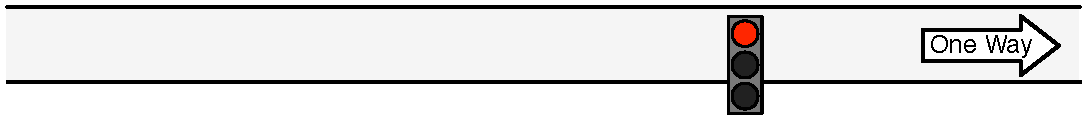
\includegraphics[width=.6\textwidth]{images/road-red.pdf}	
\end{center}


\item To model a light turning from \textbf{\textcolor{green}{green}} to \textbf{\textcolor{red}{red}}, we need to be more creative. What is an initial car density $\rho(x,0) = \rho_0(x)$ that will guarantee incoming cars have to stop at the red light?

	
\end{parts}
	
\end{slide}





\begin{slide}
\question \label{traffic:red}

\begin{problem}[Traffic flow scenario]

We want to solve the following traffic flow problem:
\begin{align*}	
	& \rho_t + v_{\max} \left( 1 - \frac{2 \rho}{\rho_{\max}}\right) \rho_x = 0  \tag{Traffic flow model} \\
	& r(x,0) = f(x) = 
		\begin{cases}
			\rho_{\min}	& \text{ for } x<0\\
			\rho_{\max}	& \text{ for } x>0
		\end{cases}
\end{align*}

Consider the following parameters: 
\begin{itemize}
	\item $v_{\max}=60$
	\item $\rho_{\max} = 120$
	\item $\rho_{\min} = 20$
\end{itemize}
\end{problem}


\begin{parts}
	\item What are the moving observers (characteristics) $x(t)$ for this problem?
	\item What is the density $\rho(x,t)$?
	\item Sketch the characteristics and mark the values of $\rho$ on the same graph below.
	
	\begin{center}
	\begin{tikzpicture}
		\draw[-latex] (0,-0.5) -- (0,2) node[left] {$t$};
		\draw[-latex] (-2.5,0) -- (2.5,0) node[above] {$x$};	
	\end{tikzpicture}
	\end{center}

	
	\item What is $\rho(0,2)$?
\end{parts}

	
\end{slide}



\addcontentsline{toc}{subsubsection}{Shockwaves and Rankine-Hugoniot condition}


\begin{slide}
\question
When characteristics intersect, this means that the solution \textbf{cannot be continuous}.

So we need to find a \textbf{discontinuous} solution.

\begin{itemize}
\item Assume that the discontinuity forms a curve $x_s(t)$.
\end{itemize}

\begin{center}
	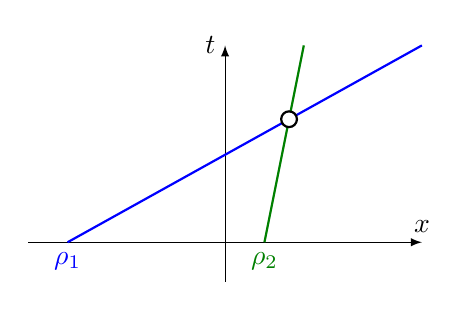
\begin{tikzpicture}
		\draw[-latex] (0,-0.5) -- (0,2.5) node[left] {$t$};
		\draw[-latex] (-2.5,0) -- (2.5,0) node[above] {$x$};	
		\draw[thick,blue] (-2,0) node[below] {$\rho_1$} -- (2.5,2.5);
		\draw[thick,green!50!black] (0.5,0) node[below] {$\rho_2$} -- (1,2.5);
		\draw[thick, fill=white] (0.8125,1.5625) circle (0.1);
	\end{tikzpicture}	
	\qquad 
	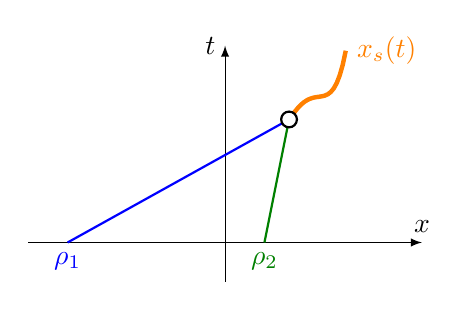
\begin{tikzpicture}
		\draw[-latex] (0,-0.5) -- (0,2.5) node[left] {$t$};
		\draw[-latex] (-2.5,0) -- (2.5,0) node[above] {$x$};	
		\draw[thick, blue] (-2,0) node[below] {$\rho_1$} -- (0.8125,1.5625);
		\draw[thick, green!50!black] (0.5,0) node[below] {$\rho_2$} -- (0.8125,1.5625);
		\draw[orange, ultra thick, variable=\x,domain=0:0.72,samples=20] plot({\x+0.8125},{1.5625+0.4*\x-9*\x*\x*\x+\x+12*\x*\x*\x*\x}) node[right] {$x_s(t)$};
		\draw[thick, fill=white] (0.8125,1.5625) circle (0.1);
	\end{tikzpicture}	
\end{center}



\begin{parts}
	\item What should the discontinuity $x_s(t)$ be?
\end{parts}
	
\end{slide}


\begin{slide}
\question

We need to step back for a moment and review some Calculus.

Consider a function
\[
F(x) = \int_0^z g(x) ~dx
\]
and consider a differentiable function $h(t)$.

\begin{parts}
	\item What is $F'(z)$?
	\item What is $F'\big(g(t)\big)$? 
	 	\qquad What is $\left[ F\big(h(t)\big) \right]'$?

	\item What is $\displaystyle \left[ \int_0^{h(t)} g(x) ~dx \right]'$?
		\qquad  What is $\displaystyle \left[ \int_{h(t)}^1 g(x) ~dx \right]'$?

\end{parts}

\end{slide}



\begin{slide}
\question
We need to go back to the derivation of the traffic flow model.

We had the following:
\[
\frac{d}{dt} \left[ \int_a^b \rho(x,t) ~dx \right] = \phi(a,t) - \phi(b,t)
\]

We then took the derivative inside the integral, because we assumed that the density $\rho$ was differentiable (thus continuous). Now we know it is not, so we must break up the interval of integration into ``chunks'' where $\rho$ is continuous.

We now assume that $\rho(x,t)$ is discontinuous across $x=x_s(t)$.

\begin{parts}
	\item Expand the left-hand side of the equation into integrals with continuous integrands.
	\item We know that $\phi = \phi(\rho)$. Take the limits
	\[ a \to \big(x_s(t)\big)^- \quad \text{ and } \quad b \to \big(x_s(t)\big)^+ \]
	and obtain an ODE for $x_s(t)$.
	
	This ODE is called the \textbf{Rankine-Hugoniot shockwave condition}.
	
\end{parts}
	
\end{slide}


\begin{solution}

\begin{slide}

\begin{parts}

\item We have
\begin{multline*}	
	\frac{d}{dt} \left[ \int_a^b \rho(x,t) ~dx \right] \\
		= \frac{d}{dt} \left[ \int_a^{x_s(t)} \rho(x,t) ~dx + \int_{x_s(t)}^b \rho(x,t) ~dx \right]
\end{multline*}

Using the previous exercise, we get
%\[\rho\big(x_s^-(t),t\big) x_s'(t) - \rho\big(x_s^+(t),t\big) x_s'(t)	+ \int_a^b \rho_t(x,t) ~dx \]
\[
\left[\rho\big(x_s^-(t),t\big)- \rho\big(x_s^-(t),t\big) \right] x_s'(t) + \int_a^b \rho_t(x,t) ~dx
\]

	\item Let us define the following
	\begin{itemize}
		\item $\displaystyle\rho^-(t) = \lim_{x \to x_s^-(t)} \rho(x,t)$
		\item $\displaystyle\rho^+(t) = \lim_{x \to x_s^+(t)} \rho(x,t)$
	\end{itemize}
	
%	Then we have
%	\[
%	\left[\rho\big(x_s^-(t),t\big)- \rho\big(x_s^-(t),t\big) \right] x_s'(t) + \int_a^b \rho_t(x,t) ~dx
%		= \phi\big(\rho(a,t)\big)	 - \phi\big(\rho(b,t)\big)
%	\]
	So when we take the limits, we obtain
	\[
		( \rho^-(t) - \rho^+(t)) x_s'(t) = \phi(\rho^-(t)) - \phi(\rho^+(t)) 
	\]
	We get
	\[
		x_s'(t) = \frac{\phi(\rho^-) - \phi(\rho^+)}{\rho^- - \rho^+}
	\]

	This condition is called the \textbf{Rankine-Hugoniot shockwave condition}.
\end{parts}

\end{slide}
\end{solution}




\begin{slide}
\question

\begin{parts}
	\item Use the Rankine-Hugoniot shockwave condition to find the full solution of Exercise \ref{traffic:red}.
	
	
	\item Compare the solution to the numerical solution using the Lax-Friedrichs method in \href{https://utoronto.syzygy.ca/jupyter/user-redirect/git-pull?repo=https://github.com/bigfatbernie/IBLMathModeling&subPath=book/python/traffic_flow_LaxFriedrichs.ipynb}{\tt traffic\_flow\_LaxFriedrichs.ipynb}.
	
	Note that to use this method, we wrote the PDE as
	$ \rho_t + \big( \phi(\rho) \big)_x = 0 $
	with $\phi(\rho) = v_{\max} \left( 1 - \frac{\rho}{\rho_{\max}}\right) \rho$.
	
	\textit{Note also that the method is very sensitive to the choice of $\Delta x$ and $\Delta t$: it only works when $\frac{\Delta t}{\Delta x}$ is small enough.}
		
	\begin{minipage}{.55\textwidth}
		\item Trace the paths of the cars starting at $x_0 = -10, -5, 0, 2.5$.
	\end{minipage}\hfil 
	\begin{minipage}{.4\textwidth}
	\begin{tikzpicture}[scale=0.85]
		\draw[-latex] (0,-0.1) -- (0,2) node[left] {$t$};
		\draw[-latex] (-2.5,0) -- (2.5,0) node[above] {$x$};	
	\end{tikzpicture}
	\end{minipage}
	
	
	\item What happens when cars slow down gradually? Find the solution for the initial condition
	\[	r(x,0) = f(x) = 
		\begin{cases}
			\rho_{\min}	& \text{ for } x<-1\\
			\rho_{\max} + (\rho_{\min}-\rho_{\max})x & \text{ for } -1 \leq x \leq 0 \\ 
			\rho_{\max} 	& \text{ for } x>0
		\end{cases}
	\]
	
	
	\item How would the model change if there is an on-ramp at $x=0$? 
	
\end{parts}

	
\end{slide}


\begin{solution}
\begin{slide}

\begin{parts}

\item The Rankine-Hugoniot condition yields:
\[
x'_s(t) = \frac{\phi(20) - \phi(120)}{20-120} = -\frac{1000 - 0}{100} = -10
\]
where we recall that $\displaystyle\phi(\rho) = v_{\max} \left( 1 - \frac{\rho}{\rho_{\max}}\right) \rho = 60 \left(1 - \frac{\rho}{120}\right) \rho$.

We also know that the discontinuity starts at the point $(x,t) = (0,0)$, so 
\[
x_s(t) = -10t
\]

\begin{minipage}{.5\textwidth}
This means that the solution is
\[
\rho(x,t) = 
	\begin{cases}
		\rho_{\min} & \text{ for } x < x_s(t) \\
		\rho_{\max} & \text{ for } x > x_s(t)
	\end{cases}
\]

In practice this means that cars are accumulating behind the traffic sign ($\rho_{\max}$) means cars are stopped.
The cars are accumulating at the speed of $10$ km/h.
\end{minipage}
\hfill
\begin{minipage}{.4\textwidth}
	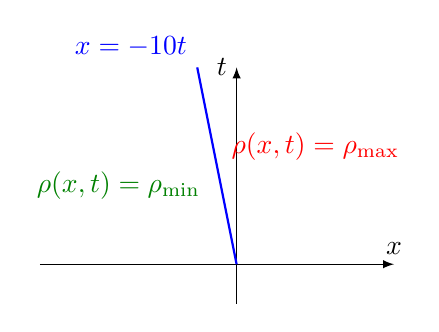
\begin{tikzpicture}
		\draw[-latex] (0,-0.5) -- (0,2.5) node[left] {$t$};
		\draw[-latex] (-2.5,0) -- (2,0) node[above] {$x$};	
		\draw[thick, blue] (0,0) -- ({-2.5/5},2.5) node[above left] {$x=-10t$};
		\draw[green!50!black] (-1.5,1) node {$\rho(x,t) = \rho_{\min}$};
		\draw[red] (1,1.5) node {$\rho(x,t) = \rho_{\max}$};
%		\draw[thick,blue] (-2,0) node[below] {$\rho_1$} -- (2.5,2.5);
%		\draw[thick,green!50!black] (0.5,0) node[below] {$\rho_2$} -- (1,2.5);
%		\draw[thick, fill=white] (0.8125,1.5625) circle (0.1);
	\end{tikzpicture}	
\end{minipage}

\end{parts}
	
\end{slide}	
\end{solution}


\begin{solution}
\begin{slide}
\begin{parts}
\setcounter{partsitem}{1}
\item When we run the numerical solution \href{https://raw.githubusercontent.com/bigfatbernie/IBLMathModeling/main/book/images/traffic_flow-60.mp4}{(click here to see an animation)}, we get the following:

\hfil \begin{tabular}{c}
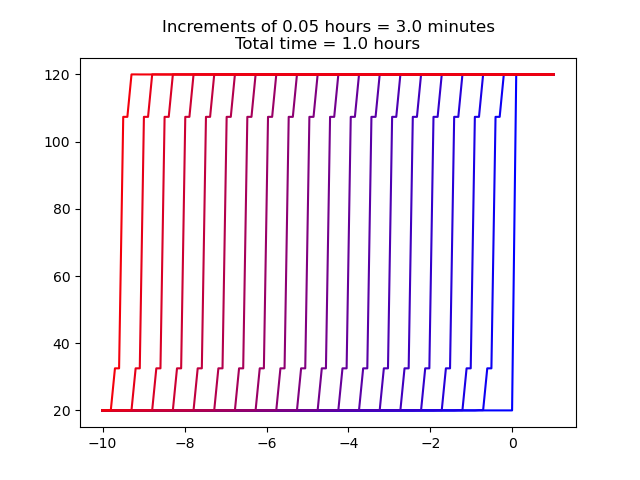
\includegraphics[width=.35\textwidth]{images/traffic_flow-60-deltax110.png} \\[-8pt]
larger $\Delta x$ and $\frac{\Delta t}{\Delta x} = 0.02$
\end{tabular}
\hfil \begin{tabular}{c}
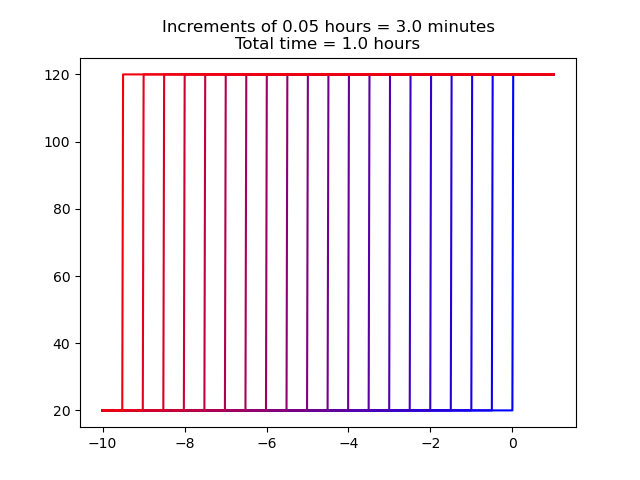
\includegraphics[width=.35\textwidth]{images/traffic_flow-60-deltax550.png} \\[-8pt]
smaller $\Delta x$ and $\frac{\Delta t}{\Delta x} = 0.1$
\end{tabular}

If the resolution in $x$ is not good enough, then we see some artifacts from the numerical approximation.

We can estimate the speed of the shockwave: it takes 4 time-steps to get to from $x=0$ to $x=-2$:
\begin{itemize}
	\item Speed of the shockwave $= \frac{2}{4 \cdot (0.05)} = 10$ km/h.
\end{itemize}

\end{parts}
\end{slide}

\begin{slide}

\begin{parts}
\setcounter{partsitem}{2}
\item 	 \hfill 

\def\tmax{0.3}
\begin{center}
	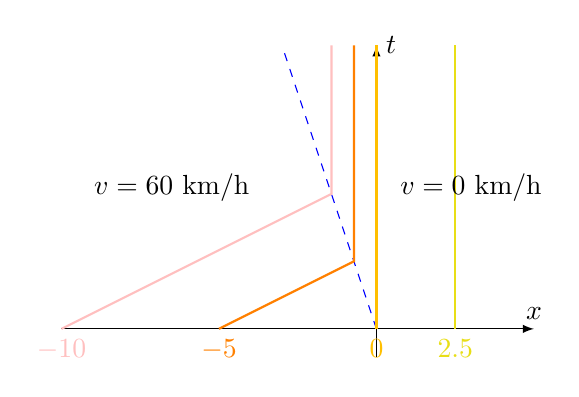
\begin{tikzpicture}[xscale=0.40,yscale=12]
		\draw[-latex] (0,{-\tmax/10}) -- (0,\tmax) node[right] {$t$};
		\draw[-latex] (-10,0) -- (5,0) node[above] {$x$};	
    	\draw[blue,dashed] (0,0) -- ({-\tmax*10},\tmax);
        \draw[yellow!90!black, thick] (2.5,0) node[below] {$2.5$} -- (2.5,\tmax);
        \draw[orange!50!yellow, thick] (0,0)  node[below] {$0$} -- (0,\tmax);
		\draw[orange, thick] (-5,0) node[below] {$-5$} -- ({-5+5*60/70},{5/70}) -- ({-5+5*60/70},\tmax);
    \draw[pink, thick] (-10,0) node[below] {$-10$} -- ({-10+10*60/70},{10/70}) -- ({-10+10*60/70},\tmax);
        \draw (-6.5,{\tmax/2}) node {$v = 60$ km/h};
        \draw (3,{\tmax/2}) node {$v = 0$ km/h};
	\end{tikzpicture}
\end{center}

Here is an animation of the solution: \href{https://raw.githubusercontent.com/bigfatbernie/IBLMathModeling/main/book/images/traffic_flow-animation.mp4}{traffic_flow-animation.mp4}



\item In this case, the shockwave doesn't start at $t=0$, but when the characteristics meet for the first time.

\end{parts}
	
\end{slide}
	
\end{solution}







